\documentclass{article}
\usepackage[utf8]{inputenc}
\usepackage{graphicx}
\usepackage{amsmath}
\usepackage{amssymb}
\usepackage{makecell,tabularx}
\usepackage{hyperref}
\hypersetup{colorlinks,urlcolor=blue}
%% or
% \hypersetup{colorlinks=false,pdfborder=000}

% hack into hyperref
\makeatletter
\DeclareUrlCommand\ULurl@@{%
  \def\UrlFont{\ttfamily\color{blue}}%
  \def\UrlLeft{\uline\bgroup}%
  \def\UrlRight{\egroup}}
\def\ULurl@#1{\hyper@linkurl{\ULurl@@{#1}}{#1}}
\DeclareRobustCommand*\ULurl{\hyper@normalise\ULurl@}
\makeatother

\graphicspath{ {images/} }

\title{Coursera Notes}
\author{Siavash Aslanbeigi}
\date{April 2018}

\begin{document}

\maketitle

\section{Introduction}
\subsection{Welcome}
Machine learning is a collection of techniques which allow computers to learn from data to complete tasks, instead of being explicitly programmed to do so.The ranking which Google uses for search results is a machine learning algorithm. Spam filters are also learning algorithms; it would be impossible to list all possible spam emails one could receive. Machine learning grew out of work in Artificial Intelligence (AI). There are many tasks for which we need machines to learn on their own. Some modern applications of machine learning include:
\begin{itemize}
    \item Database mining: growth of automation/web has resulted in much larger data sets which need to be understood. Examples include web click data, medical records, etc.
    \item Handwritten digit recognition. It is surprisingly easy for humans to recognize hand-written digits, even though they could be written in many different ways. This problem is hard to solve by explicitly programming the computer to recognize shapes.
    \item Natural Language Processing (NLP). This is effort to make computers understand text.
    \item Self-customizing programs, such as Netflix product recommendations.
    \item Understanding the human brain. How is it that we humans learn?
\end{itemize}

\subsection{What is machine learning?}
Some definitions of machine learning:
\begin{itemize}
    \item Arthur Samuel (1959): Field of study that gives computers the ability to learn without being explicitly programmed. Samuel built a Checkers playing program where the computer would learn from playing tens of thousands of games against itself. This was the world's first self-learning program.
    \item Tom Mitchell (1998): A computer program is said to learn from experience E with respect to some task T and some performance measure P, if its performance on T, as measured by P, improves with experience E.
\end{itemize}
There are two main types of machine learning algorithms: supervised-learning and unsupervised learning.

\subsection{Supervised Learning}
Supervised learning is the most common type of machine learning problem. The name \textbf{supervised} comes from the fact that the training samples (i.e. our data) contain the "right answers". In other words, for a set of inputs, we know what the output should be. Suppose we have the following data for prices of houses:

\begin{figure}[ht]
\centering
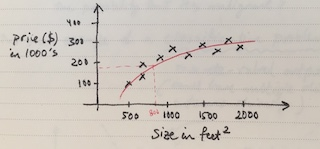
\includegraphics[scale=0.8]{images/intro/house-prices.jpg}
\caption{Predicting house prices.}
\label{into-house-prices}
\end{figure}

What is the price of a house which is $800 \text{ft}^2$? Although none of the houses in our data set have that size, we could make a prediction by fitting a curve through the data points, as shows in Figure \ref{into-house-prices}.

Supervised learning algorithms fall in two broad categories:
\begin{itemize}
    \item \textbf{Regression}: output values are continuous, for instance, predicting house prices, stock prices, etc.
    \item \textbf{Classification}: output values are discrete, for instance whether or not a tumor is malignant or benign.
\end{itemize}

Suppose we have a data set about breast tumors: we are given the size of each tumor, age of the patient, and whether or not it's malignant.

\begin{figure}[ht]
\centering
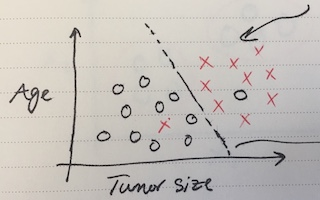
\includegraphics[scale=0.8]{images/intro/tumor.jpg}
\caption{Predicting whether new tumor is malignant or benign. Circles denote benign tumors, and Xs malignant ones.}
\label{intro-tumor}
\end{figure}

Given a new tumor, we'd like to be able to predict whether or not it's malignant or benign. This is an example of a classification problem, since the output values are discrete (we can assign $0$ to benign tumors, and $1$ to malignant ones.) The learning algorithm may decide that the line drawn in Figure \ref{intro-tumor} separates benign and malignant tumors.

\subsection{Unsupersived Learning}
In supervised learning, the training samples tell us the correct outputs for a set of inputs. We then seeks to predict the output for new examples. Unsupervised learning is different in that we not given the right answers. It's more like, here's a data set, find some structure in it. For instance, a learning algorithm may tell us that in Figure \ref{intro-clustering} most of the data is concentrated in two different regions,those which are circled. This is an example of a clustering algorithm.

\begin{figure}[ht]
\centering
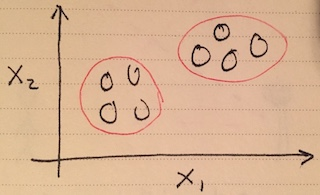
\includegraphics[scale=0.8]{images/intro/clustering.jpg}
\caption{Clustering algorithm.}
\label{intro-clustering}
\end{figure}

A real-life application of clustering is Google News, which looks at thousands of news and groups similar ones together. For instance, it would recognize that these articles from different sources are about the same topic and clusters them together:

\begin{itemize}
    \item The Source: BP kills Macondo, but its legacy lives on.
    \item CNN: Well is dead, but much Gulf Coast work remains.
    \item Guardian: BP oil spill costs nearly $\$10$bn dollars.
\end{itemize}

How remarkable is this? Here's another example of an unsupervised learning algorithm: the cocktail party problem, demonstrated in Figure \ref{intro-cocktail}.

\begin{figure}[ht]
\centering
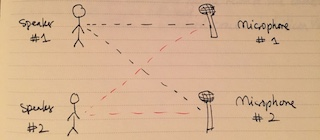
\includegraphics[scale=0.8]{images/intro/cocktail.jpg}
\caption{Cocktail party problem.}
\label{intro-cocktail}
\end{figure}

Two people are talking at the same time. In microphone 1, the sound of speaker 1 is recorded more loudly than speaker 2, simply because speaker 1 is closer to microphone 1, and vice versa for microphone 2. If the volume offsets are pronounced enough, a human would easily recognize by listening to the recording of microphones 1 and 2 that there are two speakers, and even what each of them is saying. The amazing thing is that there are unsupervised learning algorithms that are capable of doing the same. Based on the volume offsets, they recognize the structures of the two speakers sounds and are able to separate them out.


\section{Linear regression with one variable}
Consider a \textit{training set} (data set which we'll use to fit parameters of our model, or \textit{train} our model) for house prices in Portland, OR:

\begin{center}
\begin{tabular}{ |c|c| } 
 \hline
 Size ($\text{ft}^2$) (x) & Price ($\$1000$) (y) \\
 \hline
 2104 & 460 \\
 1416 & 232 \\
 1534 & 315 \\
 852 & 178 \\
 \vdots & \vdots \\
 \hline
\end{tabular}
\end{center}

Our job is to learn from this data how to predict prices of houses as a function of their size. This is a supervised learning problem, because our training set contains the right answers: for every input (house size), we know the right output (house price). Moreover, this is a regression problem, because the output variable (house price) is continuous. Figure \ref{linreg-bigpic} shows the picture of how we will tackle this problem: given the training set, our learning algorithm will spits out a function $h$, called the \textit{hypothesis} function, which can estimate the price of a house given its size.

\begin{figure}[ht]
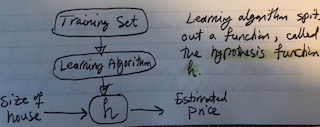
\includegraphics[scale=0.8]{images/lin_reg/big-picture.jpg}
\caption{Big picture.}
\label{linreg-bigpic}
\end{figure}

\subsection{Model Representation}
How do we represent $h$? We start with the simplest function possible and consider more complex models later:
\begin{equation}
    h_{\theta}(x) = \theta_0 + \theta_1 x.
    \label{linreg-eq:univar-hypothesis}
\end{equation}
This function assumes a linear relationship between the size of a house $x$ and its price $h_{\theta}(x)$. It is sometimes referred to as \textit{univariate linear regression}, because it is a function of a single variable (size of house) and is linear. We will come up with a learning algorithm that uses the training set to estimate the coefficients $\theta_0$ and $\theta_1$. With that at our disposal, we can predict the price of a house given its size. 


\subsection{Cost function}
What values of $\theta_0$ and $\theta_1$ provide the best "fit" to our training? Let's start by establishing notation:
\begin{itemize}
    \item $m$: Number of training examples.
    \item $x$: Input variable/feature (size of house).
    \item $y$: Output variable/target variable (price of house).
    \item $(x^{(i)}, y^{(i)})$: $i^{\text{th}}$ training example (size and price of a house in our training set).
\end{itemize}

For a given house size $x^{(i)}$ in our training set, we know the correct house price $y^{(i)}$. It then makes sense to pick $\theta_0$ and $\theta_1$ so that $h_{\theta}(x^{(i)})$ is as close to $y^{(i)}$ as possible. Realistically, we cannot tune $\theta_0$ and $\theta_1$ so that $h_{\theta}(x^{(i)})=y^{(i)}$ for all examples, since we only have two parameters to play with but many more examples ($m \gg 2$) to fit. As a result, we need to strike a balance across all examples, so that the collective prediction error $|h_{\theta}(x) - y|$ on the training set is minimized. To that end, consider the following function, called the \textit{cost function}:

\begin{align}
    J(\theta_0, \theta_1) &= \frac{1}{2m}\sum_{i=1}^{m}(h_{\theta}(x^{(i)}) - y^{(i)})^2
    \label{linreg-eq:costfunc}\\
    &= \frac{1}{2m}\sum_{i=1}^{m}(\theta_0 + \theta_1 x^{(i)} - y^{(i)})^2
    \label{linreg-eq:univar-costfunc}
\end{align}
Given $\theta_0$ and $\theta_1$, it computes the sum of (squared) prediction errors across all training examples. (It also normalizes the sum by $2m$, but that's only for mathematical convenience.) We can think about $J$ as measuring the \textit{cost} of the model's predicted house prices deviating from actual house prices in the training set. So, it makes sense to pick the values of $\theta_0$ and $\theta_1$ that minimize $J$. Figure \ref{linreg-fig:costfunc} shows the correspondence between minimizing $J$ and getting a better fit to to the training set. 

\begin{figure}[ht]
\centering
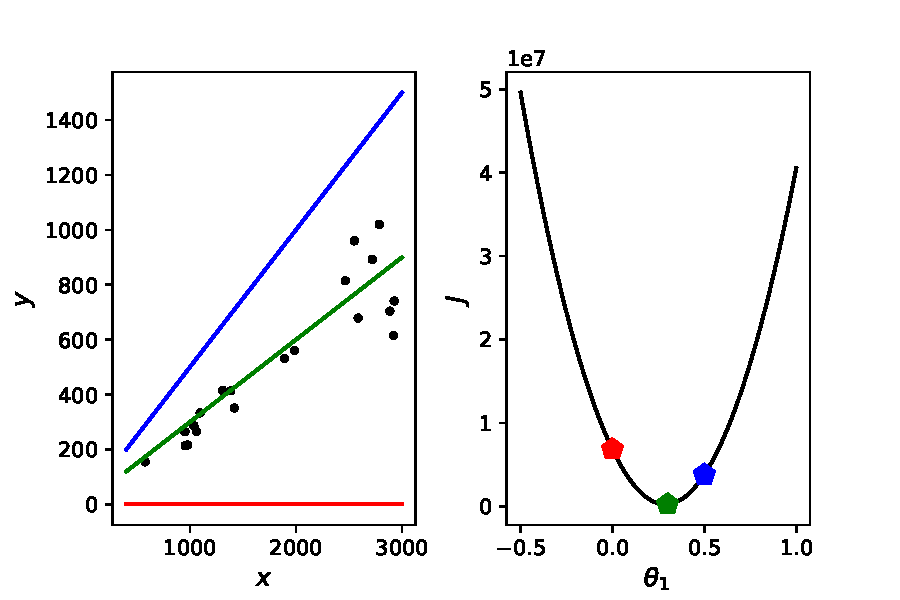
\includegraphics[scale=0.7]{images/lin_reg/costfunc.pdf}
\caption{Correspondence between minimizing the cost function and getting a better fit to data. The following model is used to fit the data: $h_{\theta}(x) = \theta_1 x$. Black dots on the left show the training set. The right figure shows the cost function $J(\theta_1)$. Every dot on the right figure corresponds to a line of the same color on the left figure. We see that the closer $\theta_1$ is to $J$'s minimum, the better the fit to data is.}
\label{linreg-fig:costfunc}
\end{figure}

Why cost function \eqref{linreg-eq:univar-costfunc} and not some other one? There are plenty of other cost functions whose minimization would also lead to a good fit of data. For linear regression, though, \eqref{linreg-eq:univar-costfunc} does have some desirable mathematical properties. First of all, $J$ is a quadratic function of $\theta_0$ and $\theta_1$, i.e. it's a paraboloid. As a result, it doesn't have any local minima, only a global one. This makes minimization a much easier task. Secondly, as we will show in the next section, minimization of $J$ can be carried out analytically.


\subsection{Minimizing the cost function}
The global minimum of $J$ occurs where its gradient is zero:
\begin{align*}
    \frac{\partial J}{\partial\theta_0} &= \frac{1}{m}\sum_{i=1}^{m}(\theta_0 + \theta_1 x^{(i)} - y^{(i)}) = 0 \\
    \frac{\partial J}{\partial\theta_1} &= \frac{1}{m}\sum_{i=1}^{m}(\theta_0 + \theta_1 x^{(i)} - y^{(i)})x^{(i)} = 0.
\end{align*}
Thus, we have to solve the following system of linear equations
\begin{align*}
    m \theta_0 + \left[\sum_{i=1}^{m}x^{(i)}\right]\theta_1 &= \sum_{i=1}^{m} y^{(i)}\\
    \left[\sum_{i=1}^{m}x^{(i)}\right] \theta_0 + \left[\sum_{i=1}^{m}\left(x^{(i)}\right)^2\right]\theta_1 &= \sum_{i=1}^{m} x^{(i)}y^{(i)},
\end{align*}
the solution to which is given by
\begin{equation}
\begin{pmatrix}
\theta_0\\
\theta_1
\end{pmatrix}
=
\begin{pmatrix}
m & \sum_{i=1}^{m}x^{(i)}\\
\sum_{i=1}^{m}x^{(i)} & \sum_{i=1}^{m}\left(x^{(i)}\right)^2
\end{pmatrix}^{-1}
\begin{pmatrix}
\sum_{i=1}^{m}y^{(i)}\\
\sum_{i=1}^{m}x^{(i)}y^{(i)}
\end{pmatrix}.
\label{linreg-eq:univar-sol}
\end{equation}
We have solved the problem we posed in the beginning of this section. Given the training set, we can use \eqref{linreg-eq:univar-sol} to estimate $\theta_1$ and $\theta_2$, and then make predictions using \eqref{linreg-eq:univar-hypothesis}.


\section{Linear regression with multiple variables}
In the previous section, we wanted to predict the price of a house as a function of its size. Of course, there are many more factors would could affect house prices:

\begin{center}
\begin{tabularx}{\linewidth}{ |l|X|X|X|l| } 
 \hline
 \thead{Size (ft$^2$) ($x_1$)} &
 \thead{Number of\\ bedrooms ($x_2$)} &
 \thead{Number of\\ floors ($x_3$)} &
 \thead{Age of home\\ (years) ($x_4$)} &
 \thead{Price (\$1000) (y)}\\
 \hline
 2104 & 5 & 1 & 45 & 460 \\
 1416 & 3 & 2 & 40 & 232 \\
 1534 & 3 & 2 & 30 & 315 \\
 852 & 2 & 1 & 10 & 178 \\
 \vdots & \vdots & \vdots & \vdots & \vdots\\
 \hline
\end{tabularx}
\label{linreg-tab:houseprice}
\end{center}

The independent variables $x_1-x_4$ (e.g. size of house, number of bedrooms, etc), which we think the output variable depends on, are called \textit{features}. In this section, we will generalize the univariate linear regression to incorporate more than just one feature.


\subsection{Model Representation}
We start by establishing notation:

\begin{itemize}
    \item $n$: Number of features.
    \item $x^{(i)}_{j}$: Value of $j$th feature in the $i$th training example.
\end{itemize}
For data shows in Table \ref{linreg-tab:houseprice}: $n=4$, $x^{(2)}_3=2$, etc. We generalize the univariate hypothesis \eqref{linreg-eq:univar-hypothesis} to a multivariate one as follows:
\begin{equation}
    h_{\theta}(x) = \theta_0 + \theta_1x_1 + \theta_2x_2 + \cdots + \theta_nx_n.
    \label{linreg-eq:multi-hypothesis}
\end{equation}
Let's establish more notation, so we can write \eqref{linreg-eq:multi-hypothesis} in matrix form:
\begin{itemize}
    \item $x_0 \equiv 1$. In other words, $x^{(i)}_0 = 1$ for all $i$.

    \item $x=
        \begin{pmatrix}
            x_0 \\
            x_1 \\
            \vdots \\
            x_n
        \end{pmatrix}
        \in \mathbb{R}^{n+1}
    $ denotes the vector of features.

    \item $x^{(i)}=
        \begin{pmatrix}
            x^{(i)}_0 \\
            x^{(i)}_1 \\
            \vdots \\
            x^{(i)}_n
        \end{pmatrix}
        \in \mathbb{R}^{n+1}
    $ denotes the vector of features for the $i$th training example. 

    \item $\theta =
        \begin{pmatrix}
            \theta_0 \\
            \theta_1 \\ 
            \vdots \\
            \theta_n
        \end{pmatrix}
        \in \mathbb{R}^{n+1}
    $ is the vector of parameters.
\end{itemize}
We have created a fictitious feature $x_0$ whose value is always set to $1$. This helps us rewrite the hypothesis function in matrix form:
\begin{equation}
    h_{\theta}(x) = \theta^Tx.
    \label{linreg-eq:multi-hypothesis-mat}
\end{equation}

\subsection{Cost function}
We will use the same cost function \eqref{linreg-eq:costfunc}, but with hypothesis \eqref{linreg-eq:multi-hypothesis}:
\begin{align}
    J(\theta) &= \frac{1}{2m}\sum_{i=1}^{m}(h_{\theta}(x^{(i)}) - y^{(i)})^2 \notag\\
    &= \frac{1}{2m}\sum_{i=1}^{m}(\theta^Tx^{(i)} - y^{(i)})^2.
    \label{linreg-eq:multi-costfunc}
\end{align}
Now $J$ is a function of $n+1$ variables ($\theta_0, \theta_1, \dots, \theta_n$), and we will need to find the vector $\theta$ that minimizes $J$. Before dealing with the minimization problem, let's rewrite $J$ in a more compact form. Consider the following definitions:
\begin{itemize}
    \item Design matrix $X$: $m \times (n+1)$ matrix whose elements are given by $X_{ij} = x^{(i)}_j$. Every row corresponds to a training example, and every column to a feature.
    \item Target vector $Y$: $m$-dimensional vector of all outputs in the training set, i.e. $Y_i=y^{(i)}$.
\end{itemize}
For data shows in Table \ref{linreg-tab:houseprice}, the design matrix and target vector are given by
\begin{equation}
    X =
    \begin{pmatrix}
        1 & 2104 & 5 & 1 & 45 \\
        1 & 1416 & 3 & 2 & 40 \\
        1 & 1534 & 3 & 2 & 30 \\
        1 & 852 & 2 & 1 & 10 \\
        \vdots & \vdots & \vdots & \vdots & \vdots \\
    \end{pmatrix},
    \qquad
    Y =
    \begin{pmatrix}
        460 \\
        232 \\
        315 \\
        178 \\
        \vdots
    \end{pmatrix}.
\end{equation}
With these definitions, we can show that $\theta^Tx^{(i)}$ is the $i$th component of the the $m$-dimensional vector $X\theta$: $\theta^Tx^{(i)}=\sum_{j=0}^n\theta_jx^{(i)}_j=\sum_{j=0}^nX_{ij}\theta_j=[X\theta]_i$. This in turn helps us write $J$ in terms of the squared norm of the vector $X\theta - Y$:
\begin{align}
    J(\theta) &= \frac{1}{2m}\sum_{i=1}^{m}(\theta^Tx^{(i)} - y^{(i)})^2\notag\\
    &= \frac{1}{2m}\sum_{i=1}^{m}([X\theta]_i - Y_i)^2\notag\\
    &= \frac{1}{2m}\sum_{i=1}^{m}[X\theta - Y]_i[X\theta - Y]_i\notag\\
    &= \frac{1}{2m}(X\theta - Y)^T(X\theta - Y).
    \label{linreg-eq:multi-costfunc-mat}
\end{align}

Why do we care to write $J$ in matrix (or sometimes called \textit{vectorized}) form? One reason is parallelization: matrix multiplication is a highly parallelizable operation. Consider $C=AB$, where $A$ and $B$ are $1000,000 \times 5$ and $5 \times 1$ dimensional, respectively. All $1000,000$ components of $C$ can be computed in parallel, because they do not depend on one another. Most programming languages have highly optimized libraries for matrix multiplication. In the following Python \href{https://github.com/siavashaslanbeigi/machine_learning/blob/master/lin_reg/matrix.ipynb}{\color{blue} example}, it's shown that a vectorized implementation of \eqref{linreg-eq:multi-costfunc-mat} is more than two orders of magnitude faster than a for-loop implementation of \eqref{linreg-eq:multi-costfunc}. This is not all due to parallelization; overhead of the for-loops itself is probably a major factor. This should, however, serve to demonstrate the importance of vectorized implementations for large data sets.

Writing expressions in matrix form also makes it easier to see when linear algebra results could be relevant. For instance, later in this section we will use the eigen-values and eigen-vectors of $X^TX$ to show that minimization of $J$ does not lead to a unique solution for $\theta$ when $m<n+1$.


\subsection{Normal equation}
Just like the univariate case, $J$ is a quadratic function of $\theta_0, \theta_1, \dots, \theta_n$, and its global minimum occurs where its gradient is zero. Let's compute the gradient of $J$ with respect to $\theta_j$:
\begin{align*}
    \frac{\partial J}{\partial \theta_j} &= \frac{1}{m}\sum_{i=1}^{m}(\theta^Tx^{(i)} - y^{(i)})x^{(i)}_j\\
    &=\frac{1}{m}\sum_{i=1}^{m}[X\theta - Y]_iX_{ij}\\
    &=\frac{1}{m}[X^T(X\theta - Y)]_j,
\end{align*}
or equivalently
\begin{equation}
    \nabla_{\theta} J = \frac{1}{m}X^T(X\theta - Y).
\end{equation}
As a sanity check, note that the dimensions of the two sides match: $\nabla_{\theta} J$ is an ($n+1$)-dimensional vector, and $X^T(X\theta - Y)$ is a multiplication between a $(n+1) \times m$ and $m \times 1$ matrix, which again is an ($n+1$)-dimensional vector. Setting the gradient to zero, we arrive at the value of $\theta$ that minimizes:
\begin{equation}
    \theta = \left(X^TX\right)^{-1}X^TY.
    \label{linreg-eq:normal}
\end{equation}
This is called the \textit{normal} equation. You should check for yourself that \eqref{linreg-eq:normal} reduces to \eqref{linreg-eq:univar-sol} when $n = 1$.

So there we have it. Given the training set in the form of the design matrix $X$ and the target vector $Y$, we can estimate $\theta$ via \eqref{linreg-eq:normal} and then use \eqref{linreg-eq:multi-hypothesis-mat} to make predictions for new examples.


\subsection{Polynomial regression}
What if our data is better modeled as a polynomial? For instance, we might think that house prices

\end{document}
